\section{Activités}


\subsection{Présentation générale}
%La supervision est l'ensemble des moyens mis en œuvre pour piloter les procédés automatisés. À Clemessy, la supervision est informatique et est surtout utilisée pour de la surveillance de systèmes et d'activités. Le projet ULI sur lequel j'ai travaillé consiste à l'automatisation et la supervision des voies ferrées d'Arcelor-Mittal Dunkerque. J'ai été chargé du secteur P2, ``Avalfer'', composé de 3 sous-secteurs : P3 (Poste 3), \gls{PN}16 (Passage à niveau numéro 16), TRI (Triangle). Chaque sous-secteur dispose d'un automate qui lui est propre et qui gérera les déplacements des \glspl{aiguille} et l'affichage des signaux. Le but premier de la supervision étant la gestion d'itinéraires pour les trains.\newline
%Comme je n'ai pas travaillé sur la partie automatisme car n'ayant pas les connaissances dans ce domaine, cette partie ne sera développée que brièvement.
%\newline
%Au cours de mon stage, mon cahier des charges variait selon mon état d'avancement. Cependant, la création de \glspl{vue} et d'objets graphiques animés a été ma charge principale. Afin de mieux comprendre ce que j'ai effectué pendant ces 9 semaines, je vous présenterai le projet sur lequel j'ai travaillé. Viendront ensuite les logiciels que j'ai utilisés tout au long de mon stage, puis j'expliquerai plus en détails mes activités et leurs avancements à la fin de mon stage. Je terminerai sur quelques réflexions personnelles. 
%\newline
\subsection {Projet}
Le projet HUBIC sur lequel j'ai travaillé est un HUB Inter-applicatif Central, ou une plateforme
d'échanges intégrée au projet X11.
Le projet X11 construit les services adaptés à l'accroissement du besoin en échanges d'informations
ainsi qu'à la diversité des modes d'échanges et à la multiplication des acteurs opérationnels
du domaine de la circulation ferroviaire. La plateforme X11 représente le socle d'échanges d'informations
permettant à l'ensemble de ses acteurs de transmettre, de partager, d'enregistrer et
de prélever de façon efficiente les informations opérationnelles relatives aux circulations ferroviaires.
La plateforme est également le support de la concertation avant décision.
HUBIC permet de faire communiquer plusieurs applications entre elles, telles que GAIA, GED,
DINAMIC, BREHAT entre autres. Ce projet fait partie de la PfGE, la Plateforme de Gestion
des Échanges, qui assure 4 grandes fonctions :
\begin{itemize}
	\item La gestion des flux "au fil de l'eau" d'un producteur à un ou plusieurs consommateurs ;
	\item La médiation entre des applications productrices et consommatrices de services ;
	\item L'alimentation du Gisement de Données Circulation ;
	\item La supervision technique et fonctionnelle des flux 
\end{itemize}

La spécification des échanges entre les différentes applications et HUBIC est découpée en 2
parties :
\begin{itemize}
\item La première technique correspondant au contrat d'interface entre HUBIC et chaque application
pour chaque sens de communication. Ce contrat est décrit dans un Dossier
d'Interface Technique ou DIT : il y en a un par application connectée à HUBIC.
\item La seconde, les traitements internes à HUBIC qui peuvent être nécessaires pour acheminer
l'information au(x) destinataire(s) : contrôle de la sollicitation de service, démultiplication
de flux (un émetteur, plusieurs destinataires), modification éventuelle de format, de
protocole. HUBIC assure également la traçabilité autant technique que fonctionnelle des
échanges, la gestion des erreurs et les possibilités de rejeu.
\end{itemize}
Pour se faire une meilleure idée, le diagramme des flux de HUBIC est représenté en figures \ref{} et \ref{} ci-dessous. Pour ne pas surcharger ce rapport, seul un unique traitement de flux sera décrit
sur les 54 existants actuellement. Prenons le traitement entre GAIA et DECLIC.
Commençons par les flux concernés. Actuellement sont concernés les flux FT031, FT032, FT033,
FT214, FT215, FT216, FT217, FT218, FT219, FT220, FT221, FT222.
Ce traitement s'effectue sous la forme d'une invocation de service à l'initiative de DECLIC.
L'application GAIA offre 25 services tels que les lignes, les communes, les départements, les
plus courts chemins,... Ces services sont sur la figure \ref{services} ci-dessous
\begin{figure}[h!]
	\centering
	
\includegraphics[width=0.7\linewidth]{img/encours}
	\caption{Services offerts par HUBIC à destination de DINAMIC}
	\label{services}
\end{figure}

Le seul acteur du domaine est le moteur de traitement des flux, c'est l'élément du HUBIC qui
interroge les services offerts par GAIA au travers de cette demi-interface.
Le seul cas d'utilisation est la consommation d'un service GAIA. Ce qui nous donne le schéma
des cas d'utilisation suivant en figure \ref{scu} :\begin{figure}[h!]
	\centering
	
\includegraphics[width=0.7\linewidth]{img/encours.png}
	\caption{Schéma des cas d'utilisation des services GAIA}
	\label{scu}
\end{figure}

Penchons-nous maintenant sur la structure des échanges de publication.
Les services sont identifiés avec un nom composé du nom de flux dans la matrice des flux, du
nom de l'application concernée par la demi-interface, un terme contextuel permettant de situer
le service et d'un éventuel numéro d'indice, chacun étant séparé par "\_". Par exemple, le flux
suivant en figure \ref{} est identifié par "FT084\_GAIA\_VOIES"
Pour la communication en requête HTTP/REST réalisée par HUBIC sur demande des applications consommatrices :
Tous les services GAIA en production sont accessibles à travers l'URI suivante :\begin{verbatim}
https://{Env.DomaineSociété}/{DomaineMetier}/{version}/{ressource}/{format}
\end{verbatim}

Par exemple, pour appeler un service GAIA exposé avec un bouchon, on utilise l'URL suivante :
https://localhost:9992/referentiel/infrastructure/gaia/v2/gares/xml
La réponse est un fichier XML formaté comme la réponse attendue pour chaque flux. Ce fichier
est ensuite modifié si nécessaire et envoyé à l'application consommatrice. Tout le processus
d'échange pour le flux FT084 est donné en figure \ref{} ci-dessous
Les messages échangés actuellement sont les PR, les TypeStructure et les gares, avec un mapping à l'identique, c'est à dire que le message de sortie de GAIA et celui d'entrée de DECLIC
doivent être formatés de la même manière, avec le même \gls{xsd}. Le module correspondant est
donc un "passe-plat", il ne modifie rien.
\subsection{Logiciels}
\subsubsection{IHM de détails techniques des flux TIBCO BusinessWorks Process Monitor}
Pour chaque échange, un identifiant unique est généré automatiquement au sein d'HUBIC.
L'identifiant d'un flux est une donnée unique et propre à chaque processus de traitement d'un
flux. Cet identifiant est sous la forme FTxxx. Un nouveau flux implique donc de définir de façon
définitive un identifiant de flux pour ce traitement.
La distinction entre les messages d'un flux s'effectue sur leur identifiant de message.
L'écran en figure \ref{} est composé de 4 vues :
\begin{enumerate}
	\item La vue principale : contient la liste de toutes les traces d'un point de vue technique.
	 \item Le menu : permet de choisir les types de flux à visualiser. \item La vue événements/processus : Contient la liste des historiques d'une trace sélectionnée dans la vue principale. \item La vue détail : contient les détails/propriétés d'une trace ou d'un historique sélectionné
\end{enumerate}
\paragraph{Vue principale : }
Les informations affichées sont les suivantes :\\
\noindent
\begin{tabularx}{\textwidth}{|c|M{4cm}|X|M{4cm}|}
	\hline
	\rowcolor{red}
	Données& Description& Valeurs possibles& Mode\\\hline\hline
	\rowcolor{grisFonce}Process Path&
	Chemin du process qui exécute le flux dans TIBCO&
	Un chemin& Consultation\\
	\rowcolor{gris}\hline
	Process Name&
	Nom du process qui exécute le flux dans TIBCO&
	Un nom& Consultation\\
\rowcolor{grisFonce}	\hline
	Job Start&
	Horodate d'entrée dans HUBIC&
	Data au format "hh :mm.ss.fff+hh :mm aaaa-mm-jj"&
	Consultation\\
	\rowcolor{gris}\hline
	MS&
	Durée du traitement du flux&
	Une durée en millisecondes& Consultation\\
	\hline
\end{tabularx}
\paragraph{Menu : }Cette vue permet à un utilisateur de choisir entre deux vues. Une vue technique et une vue métier. Dans la vue technique, il est possible de filtrer les traces selon des critères techniques comme le nom du serveur qui a traité le message, le nom du processus dans BusinessWorks,... Dans la vue métier, il est possible de filtrer les traces sur des critères fonctionnels comme le type de données métier et l'identifiant du flux.

\paragraph{Vue événements/processus :} Les informations affichées sont les suivantes :
\LTXtable{\textwidth}{table.tex}
\paragraph{Vue détail : } Les informations affichées sont les suivantes :
\LTXtable{\textwidth}{table2.tex}
\subsubsection{TIBCO Designer}
TIBCO Designer est un Graphical User Interface (GUI) facile d'utilisation permettant de
définir des "business process". Pour définir ces process, le développeur jongle entre plusieurs
fenêtres, présentes sur la figure \ref{fig:encours} ci-dessous.
\begin{figure}[h!]
	\centering
	
\includegraphics[width=0.5\linewidth]{img/encours}
	\caption{Interface TIBCO Designer}
	\label{fig:encours}
\end{figure}
\begin{enumerate}
	\item La première, le "Project Panel" est la fenêtre où toute la hiérachie du projet sera affi-
	chée, dans l'onglet "Project", comme montré ci-dessous en figure \ref{}, ainsi que toutes les
	variables globales et les process en cours de test.\\
	\begin{figure}[h!]
		\centering
		
\includegraphics[width=0.7\linewidth]{img/encours}
		\caption{Fenêtre Projet de TIBCO Designer}
		\label{fig:encours2}
	\end{figure}
	\item La deuxième, le "Design Panel", ou l'interface de développement, est la fenêtre où le
	développement s'effectue. Un process est une suite d'activités reliées entre elles. La figure
	\ref{} est un exemple de développement\\
	\begin{figure}[h!]
		\centering
		
\includegraphics[width=0.7\linewidth]{img/encours}
		\caption{Exemple de Process TIBCO}
		\label{fig:encours3}
	\end{figure}
\item La troisième, le "Configuration Panel" est la fenêtre où les activités sont paramétrées.
Cette fenêtre est constituée de plusieurs onglets :
\begin{itemize}
	\item  Configuration : Son contenu varie selon l'activité sélectionné, mais en général, c'est
	le nom de l'activité et sa description auxquels s'ajoutent un contenu plus spécifiques
	(Le nom du process appelé pour une activity "Call Process" ou le nom de la variable
	partagée pour un "Get Shared Variable", entre autres)
	\item Input Editor : Plus souvent présent pour les "Mapper", c'est l'onglet qui permet
	de donner la composition de l'entrée de l'activité, le plus souvent, un XML Schema
	Definition (XSD), ou un contrat fait à la main. Ci-dessous, en figure \ref{} et \ref{}, la
	différence entre les 2.
	\item Input : Après avoir formaté l'entrée de l'activité, il faut que l'entrée soit valide. Pour
	cela, il faut mapper les sorties des activités précédentes ou les variables globales aux
	champs requis. Comme on peut voir en figure \ref{}, le mapping peut être très lourd,
	avec des conditions sur les champs ou des boucles. Si le mapping est faux, les champs
	en cause deviennent rouges.
	\begin{figure}[h!]
		\centering
		
\includegraphics[width=0.7\linewidth]{img/encours}
		\caption{Exemple de mapping}
		\label{fig:encours4}
	\end{figure}
	\item Output Editor : C'est la même chose que pour le Input Editor, mais pour la sortie
	de l'activité.
	\item Output : Cet onglet nous affiche la sortie de l'activité. Avant le test, le format de la
	sortie est affiché. Pendant le test, nous avons la sortie en XML.
	\item Error Schemas : Surtout présent pour les activités End, celles marquant la fin du
	process. Lors d'une erreur prévue en cours de process, il est possible de générer une
	exception qui sera retournée en fin de process. Si aucun schémas n'est paramétrer,
	le process tombera en erreur.
	\item Error Output : Si le process appelé est paramétré pour pouvoir retourner une erreur,
	le format de l'erreur possible sera affiché dans cet onglet.
	\item Et d'autres onglets plus rares : tels que Advanced, Input Headers ou Output Headers
	pour une requête HTTP ou Misc pour un JMS Queue Receiver.
\end{itemize}
\item La dernière, le "Palette Panel". Le c÷ur du développement TIBCO. C'est la fenêtre
où sont répertoriés toutes les activités possibles sous TIBCO Designer. Elles peuvent
être rangées par catégories (FTP, FILE, SOAP, HTTP,...) ou en commun et par ordre
alphabétique.
\end{enumerate}

\subsubsection{SoapUI}
Autoproclamé comme "L'outil de test REST et SOAP le plus avancé au monde" (cf.
www.soapui.org), SoapUI by SMARTBEAR nous permet de créer et exécuter facilement desfonctionnalit
és automatisées, des régrssion et des test de chargement. C'est pour cette dernière
fonctionnalités que je l'utilise pour le projet. Cet outil fournit une couverture de test pour Web
services en SOAP et REST, ce qui permet de tester les modules HUBIC facilement. Selon les
modules, une requête POST ou GET est utilisée, avec souvent une Basic Authentification. La
méthode GET va juste récupérer la réponse de l'URL, tandis que la méthode POST va publier
un message (text/xml) et ve renvoyer la réponses du serveur

\subsubsection{Module d'administration de la Plateforme de Gestion des Echanges}
Le module d'administration de la PfGE permet d'administrer les modules techniques constituant
la PfGE. Ses principales fonctionnalités sont :
\begin{itemize}
	\item L'authentification des utilisateurs à l'IHM du module d'administration ;
	\item Le paramétrage des utilisateurs, des rôles et des droits d'accès aux fonctionnalités à l'IHM
	du module d'administration ;
	\item La visualisation de l'état des composants techniques de la plateforme ;
	\item Le déploiement des composants techniques de la PfGE ;
	\item La modification des paramètres techniques des composants de la PfGE ;
	\item L'arrêt et le redémarrage des composants techniques de la PfGE.
\end{itemize}
Ce module est sollicité par les administrateurs techniques de HUBIC via l'IHM d'administration.
Il permet de gérer l'ensemble des composants techniques constituant HUBIC ainsi que les
utilisateurs de l'IHM. Je l'ai surtout utilisé pour les livraisons.
\subsubsection{SVN}
%ArchestrA IDE, en figure \ref{ArchestrA}, est un autre logiciel de Wonderware, plus complexe qu'InTouch et utilisant ce dernier. ArchestrA est un logiciel de programmation orientée objet. Ce logiciel permet de se connecter à une \Gls{galaxy}, qui est un regroupement d'éléments tels que des aires, des objets définis par le développeur ou des applications InTouch. Le développement d'objets sous ArchestrA peut se rapprocher d'un langage de programmation orientée objet tel que JAVA. Prenons comme exemple la figure \ref{Java} ci-dessous.
%\begin{figure}[!h]
%	%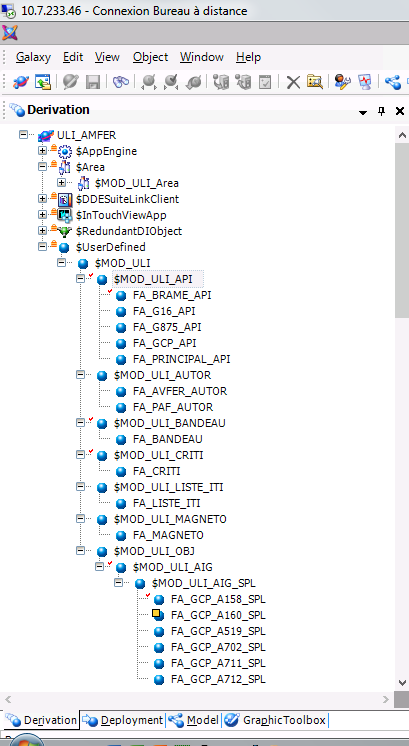
\includegraphics[scale=0.5]{Capture_Archestra_2.png}
%	\centering \caption{Exemple de dérivation d'objets.}
%	\centering
%	\label{Java}
%\end{figure}\newline
%Sur cette figure \ref{Java}, nous voyons le listing de dérivation de la \Gls{galaxy} qui peut se traduire par un arbre d'héritage en JAVA. Intéressons-nous surtout à ce que l'on pourrait appeler en Java la classe \$UserDefined. Cette ``classe'', qui est un objet sous Archestra, contient les autres objets définis pour le développement du projet. Dérivée de cet objet, la ''classe'' \$MOD\_ULI qui contient tous les objets qui seront utilisés pour la modélisation du projet, autrement dit, l'affichage des \glspl{vue}. De cet objet est dérivée la ``classe'' \$MOD\_ULI\_OBJ qui regroupe les objets qui seront placés sur la   principale du secteur Avalfer. Héritant de cette classe, on trouve une liste exhaustive de sous-classes telles que \$MOD\_ULI\_AIG qui représente les \glspl{aiguille}, \$MOD\_ULI\_BAR qui représente les barrières, \$MOD\_ULI\_PNx qui représente les passages à niveau x, \$MOD\_ULI\_VOI qui représente les voies ferrées,... On trouve ensuite les classes \$MOD\_ULI\_AIG\_SPL, \$MOD\_ULI\_AIG\_TJS et \$MOD\_ULI\_AIG\_TJD héritant de la classe \$MOD\_ULI\_AIG. Finalement, nous trouvons des instances d'objets comme FA\_GCP\_A158\_SPL qui représente donc en JAVA un objet et qui dispose de variables, de scripts et de graphiques locaux en plus de ceux hérités. Nous verrons tout cela plus en détails peu après.
%\newline Nous avons vu qu'à la différence près de dénomination entre Classe en JAVA et Objet sous ArchestrA et entre Objet en JAVA et Instance d'Objet sous Archestra, il y a héritage ou dérivation des variables, graphiques ou scripts. Nous verrons ce qu'il en est du type des variables lors de la création du menu des travaux.
%\newline
%\subsubsection{Object Viewer et SMC}
%Lors de mes tests sous ArchestrA, je me suis aidé de l'``Object Viewer`` et du ``SMC'' (System Management Console). Le premier est une fenêtre qui permet de sélectionner  les variables ArchestrA que l'on veut surveiller ou modifier facilement. C'est là où l'on peut également voir si les variables ont bien été configurées (``Quality'') et leur dernière date de mise à jour. La figure \ref{OV} montre un exemple de l'``Object Viewer''
% \begin{figure}[!h]
%	%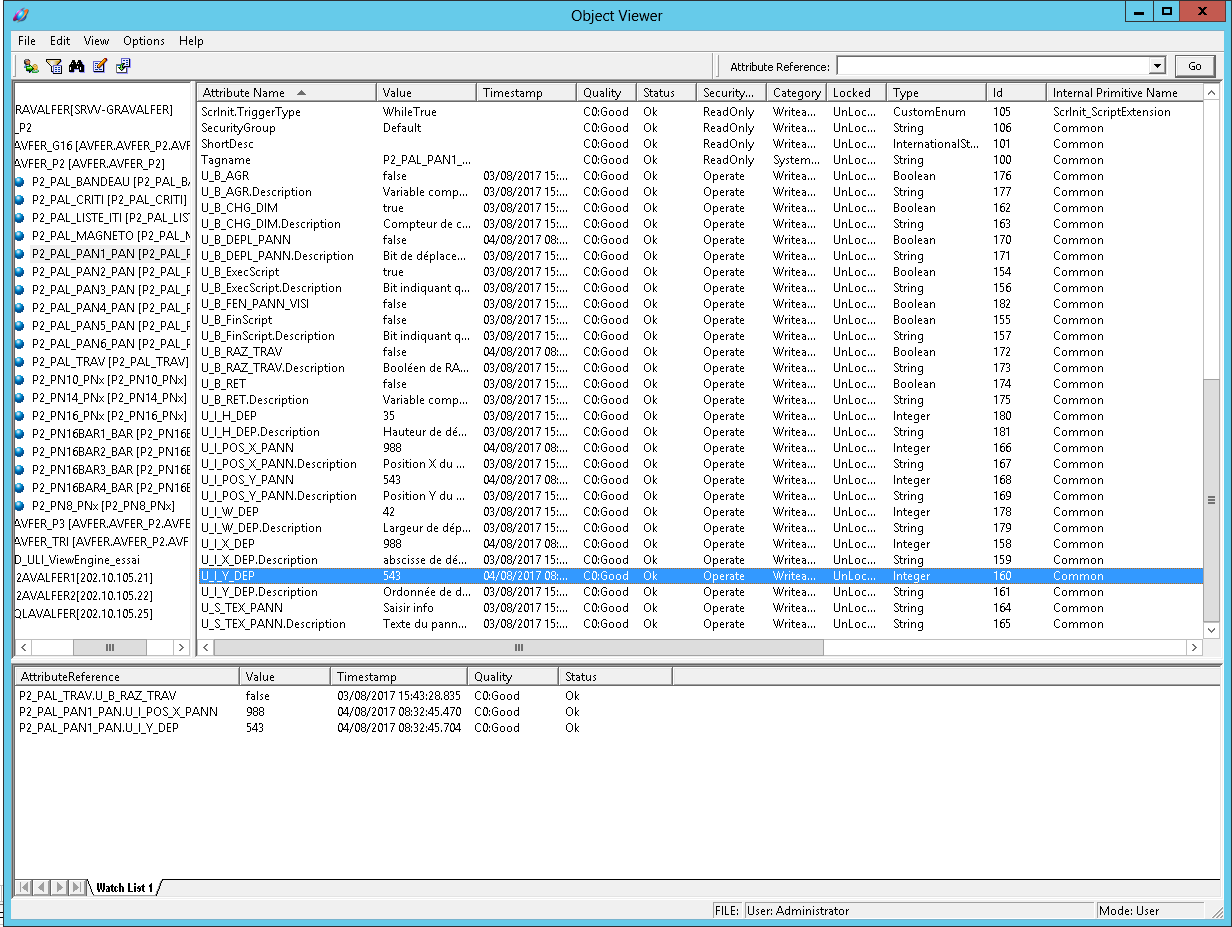
\includegraphics[width=\textwidth]{image17-1.png}
%	\centering \caption{Object Viewer.}
%	\label{OV}
%	\centering
%\end{figure}\newline
%Le second permet de voir les actions effectuées lors de la supervision. Cela peut-être des informations, en blanc, qui peuvent être demandées par le développeur avec la fonction \mbox{``LogMessage()''} qui va alors afficher ce qui est entré en paramètre, des avertissements, en jaune, lors d'erreurs qui n'empêchent pas la supervision de tourner ou des erreurs, en rouge, lorsque ces dernières sont critiques et empêchent le bon fonctionnement de la supervision, comme montré en figure \ref{SMC}.
% \begin{figure}[!h]
%	%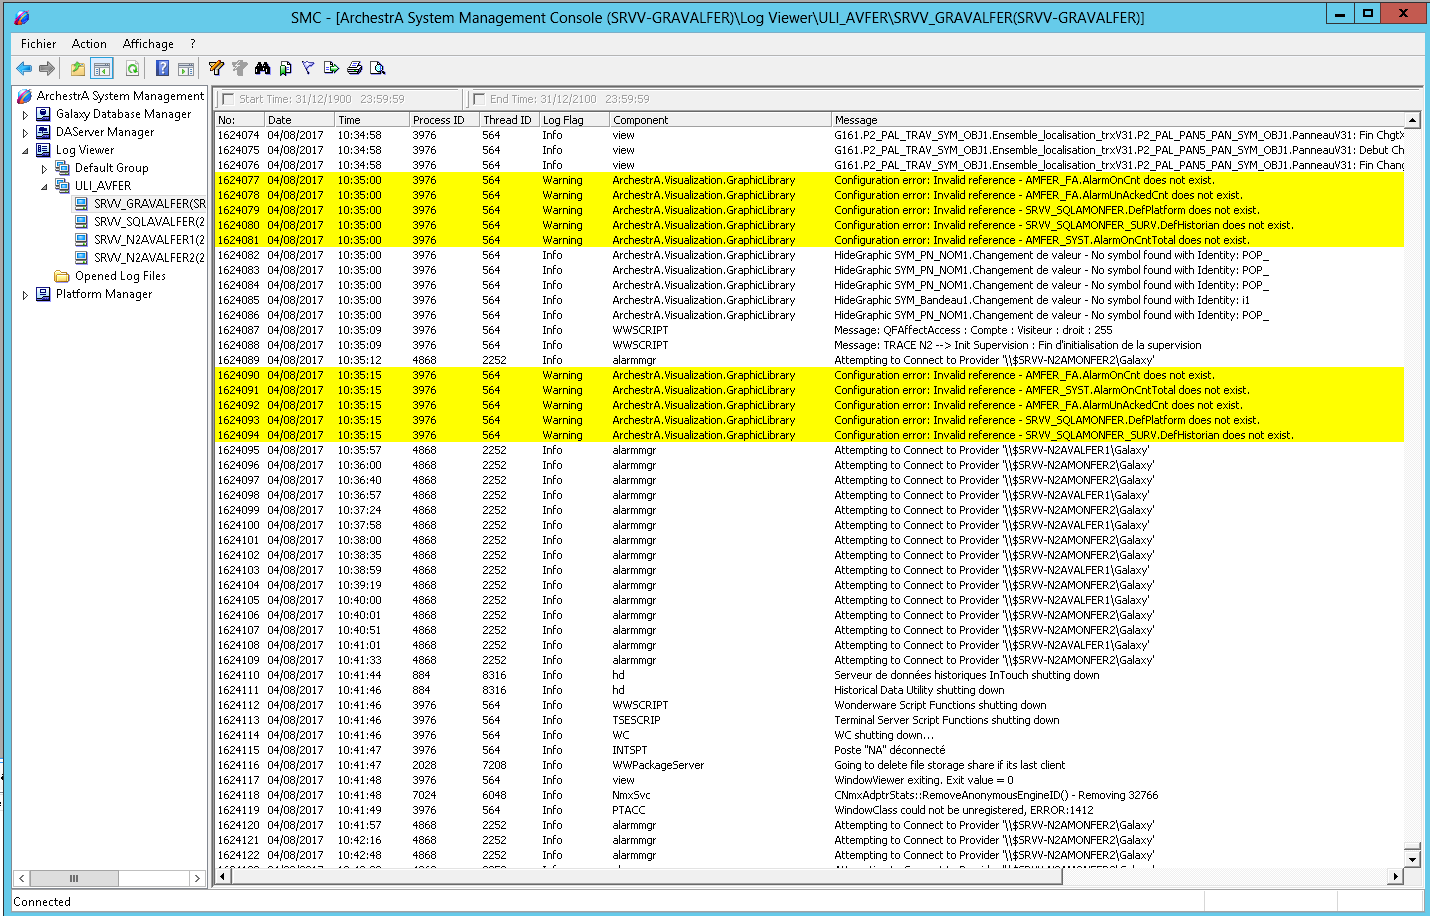
\includegraphics[width=\textwidth]{image18-1.png}
%	\centering \caption{System Management Console.}
%	\label{SMC}
%	\centering
%\end{figure}\newpage
\subsection{Activités effectuées}
Après avoir passé près de 2 semaines à lire de la documentation sur l'entreprise et sur
le projet HUBIC Pendant mon stage, j'ai travaillé sur une machine virtuelle CentOS. CentOS
(Community enterprise Operating System) est une distribution Linux stable, prévisible, gérable
et reproductive dérivée des sources et binairement compatible avec Red Hat Enterprise Linux.
Elle est également utilisée par 20\% des serveurs web Linux, ce qui en fait la 3e distribution
mondiale pour les serveurs web Linux.
\subsubsection{Prise en main de la plateforme d'intégration TIBCO ActiveMatrix BusinessWorks}
J'ai pu prendre en main TIBCO 5 et TIBCO Designer lors de mon transfert de connaissances
sur Meudon-la-Forêt, après lecture de beaucoup de documentation. J'ai commencé par
comprendre comment la plupart des activités fonctionnaient et comment les paramétrer. Travaillant
dans les web services, j'ai surtout utilisé les activités HTTP (HTTP Receiver, Send
HTTP Request et Send HTTP Response), ainsi que les activités JMS, Mapper et Parse XML
avec les modèles \gls{xsd}
\begin{figure}[!h]
	%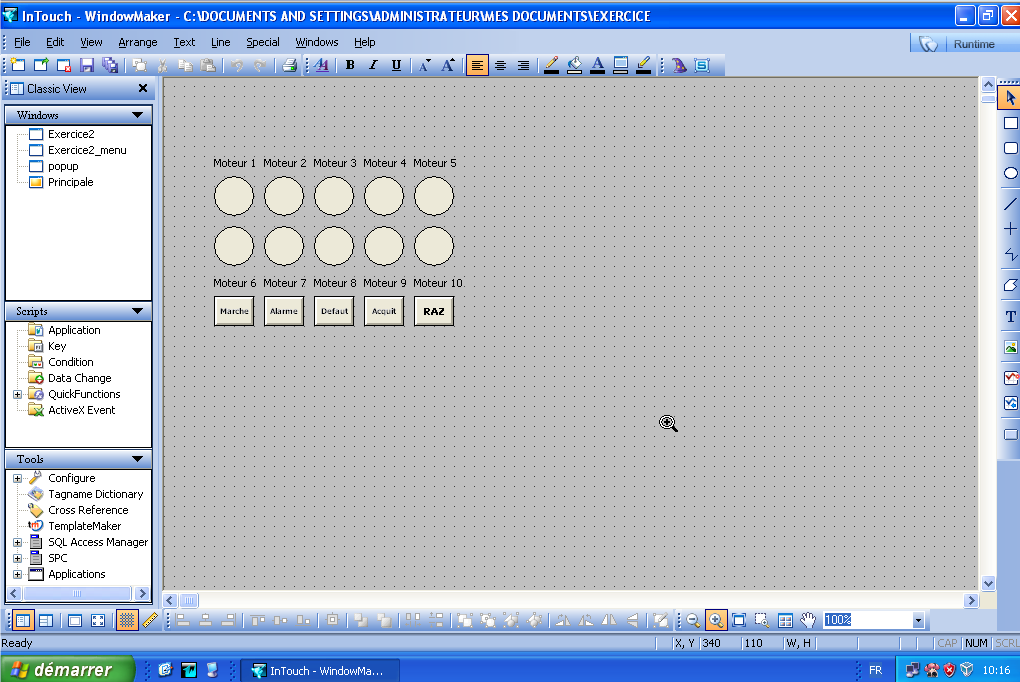
\includegraphics[height=8cm]{Capture_InTouch_3.png}
	\centering \caption{Différences entre entrée avec et sans \gls{xsd}}
	\centering
	\label{Diff}
\end{figure}

\subsubsection{POC\_GED\_MOBILE}
Mon premier projet. GED\_MOBILE est un projet annexe à GED. Un POC est un projet "test" afin de savoir si le projet est réalisable et ce que cela coûtera au client. La GED est une base de documents de la SNCF. Les services émis par la GED permettent :
\begin{itemize}
	\item De déposer/déplacer/récupérer/modifier des documents dans la GED\item De modifier les droits d'un document
\end{itemize}
Ces services n'étaient accessibles que via un ordinateur, le client a voulu étendre cela aux appareils mobiles (tablettes et téléphones) plus simple à transporter partout et permet une économie de papier pour ce qui concerne les feuilles d'intervention. Le projet consiste donc en plusieurs étapes :
\begin{enumerate}
	 \item L'utilisateur (sur mobile) effectue une demande d'autorisation et d'authentification auprès d'OpenAM. 
	 \item OpenAM authentifie l'utilisateur en interrogeant le RID. 
	 \item Si OpenAM répond à la demande par l'envoi d'un token, l'utilisateur est authentifié. 
	 \item L'utilisateur peut alors faire appel aux Web Services (en JSON) avec envoi du token dans le header. 
	 \item A la réception d'une demande, l'ESB envoie le token à OpenAM afin de vérifier que l'utilisateur est bien authentifié et que le token est toujours valide. 
	 \item Une fois l'authentification validée par OpenAM, l'ESB convertit les données reçues (JSON Ý XML) et transfert la demande a la GED en appelant le Web Servcie correspondant à cette demande. 
	 \item La GED répond à l'ESB 
	 \item L'ESB convertit les données reçues (XML \ding{213} JSON) et transfert la réponse à l'utilisateur.  
\end{enumerate}
Le projet POC\_GED\_MOBILE effectue les actions 4 à 8.

À la date du 24 mai, le projet n'est constitué que de l'authentification, sans connexion à OpenAM, soit la mise en place des process essentiels et de ceux qui suivront lors des sprints suivants et de la récupération de l'authentification.

\subsubsection {Analyse d'erreurs}
Les analyses d'erreurs sont nécessaires lorsque ce qui a été livré est tombé en erreur côté client et lorsque leur analyse a conclu à un problème côté serveur. Ma première analyse fut sur le module LEGACY. Le client a eu un problème de "bloc information circulation inexistant". Ce problème a révélé une erreur de namespace dans le XML du côté OLERON.

\subsubsection {Livraison}
Pour le projet HUBIC, la procédure de livraison est réglementée afin d'avoir toujours le même suivi sur les livraisons.
\begin{enumerate}
	\item Mise à jour du dictionnaire des BLs. Il faut ajouter une ligne correspondant à la livraison qui sera efectuée en invrémentant le numéro du Bon de livraison. 
\item Création de l'Entreprise Application ARchive. Sous TIBCO Designer, les EARs sont créés manuellement le temps que la Plateforme d'Intégration Continue soit réintroduite. Après création, il faut le zipper dans un fichier nommé hu\_sw\_ear\_NomduModule\_ja.zip et les fichiers de configuration sont à placer dans un répertoire 
\item Création des documents applicatifs. Tous les documents relatifs aux livrables doivent être générés. Il y en a sortes : 
\begin{itemize}
	\item 1 Dossier d'Intégration par module livré. 
	\item 1 chronogramme par module livré. 
	\item Le dossier de référence des DIs à jour 
	\item Le Dossier de Remontée à jour. 
\end{itemize}
Une fois ces documents générés, il faut les zipper dans l'archive DocsInstallation.zip. 
\item Ajout des livrables documentaires (optionnel). Si des documents (RDS, ods, Map des flux,...)doivent être livrés dans une archive nommée AAAAMMJJ\_LIV\_DOC\_JJmoisAAAA.zip.
\item Création de tags Subversion. Afin d'éviter tout problème lié à l'égarement des livrables, il faut systématiquement faire un répertoire dans Subversion avec le Repo Browser pour tagguer la version du trunk en cours. Il s'agit de faire un copier-coller du trunk de développement directement dans un répertoire ayant comme nom AAAAMMJJ\_Livraison. L'avantage de cette manipulation est de pouvoir récupérer le code de toute version livrée afin d'être en mesure de reproduire d'éventuelles anomalies observées chez le client, sans avoir à effectuer des recherches fastidieuses dans Subversion.
\item Création du Bon de livraison. Il s'agit de créer un répertoire avec le numéro de Bon de livraison à livrer. Le fichier se décompose en plusieurs parties. Le premier tableau liste l'ensemble des documents applicatifs, la liste des produits ainsi que la livraison documentaire. La deuxième présente les GODEC des éventuelles corrections et/ou évolutions liées à le livraison.
\item Commit Subversion de l'ensemble de la livraison dans une archive nommée AAAAMMJJ\_LIV\_HUBIC\_X.X.X\_JJmoisAAAA.zip \item Dépôt des livrables sur le serveur. Avec un logiciel comme FileZilla, il faut se connecter au serveur de livraison et déposer les livrables dans différents répertoires selon le module, les documents ou autre.
\item Dépôt des sources dans le serveur Subversion SNCF. Les sources des projets étant la propriété de la SNCF, il faudra faire un commit des sources dans leur serveur Subversion. Pour ce faire, il s'agit d'un export de la révision Subversion à livrer.\item Modifier le niveau de sécurité TLS des connecteurs HTTP de TIBCO via la configuration de l'Engine BW.\item Envoyer le mail de livraison avec en pièce jointe le Bon de livraison ainsi que l'archive comportant les documents applicatifs (ie. DocsInstalaltion.zip) \item Passer l'ensemble de GODEC au statut "Livré". Cette étape est indispensable. Toutes les GODECs mentionnées dans le Bon de livraison doivent être passées à "Livré" avant la fin de la date de livraison attendue (généralement 8h le lendemain
\end{enumerate}

\subsection{Compte-rendu des activités}
%Chaque activité que j'ai réalisée m'a permis de voir plus précisément en quoi consiste l'informatique industrielle, comment est la vie dans un open-space et surtout ce qu'est le travail dans le développement informatique. La majorité des activités qui m'ont été confiées ont été entièrement terminées dans les délais fixés. \newline
%Ma toute première activité, les exercices de prise en main d'InTouch, n'avait pas de deadline, je devais progresser à mon rythme et surtout comprendre ce que je faisais et pourquoi je le faisais. Ces exercices m'ont donc permis de prendre en main InTouch pour être plus efficace sur le développement de la supervision qui a suivi et j'ai ainsi pu m'ouvrir à mes collègues en allant leur demander de l'aide quand je ne trouvais pas mon bonheur dans le manuel d'utilisation d'InTouch. Cette activité a été faite en une semaine.\newline
%Ma deuxième activité, la création de macros Excel, m'a permis de découvrir le langage VBA et une nouvelle facette d'Excel, logiciel que je n'utilisais jamais de cette façon. J'ai également eu la possibilité d'en apprendre un peu plus sur la partie automatisation du projet et surtout de comprendre l’utilité des fichiers Excel pour la supervision. La première macro que j'ai écrit m'a pris 3 jours sur les 5 accordés, entre le temps de comprendre ce qu'est une macro, comment l'écrire, l'écrire et tester. La seconde macro, le fichier de simulation, m'a été donnée pour le début de ma quatrième semaine de stage. Cela m'a permis de mieux comprendre comment sont utilisés les fichiers Excel. J'ai réalisé la macro en six jours, sans deadline fixée car je l'utilisais pour la suite de mes activités.\newline
%Ma troisième activité, la prise en main d'ArchestrA, m'a pris 13 jours avant d'être briefé entièrement sur la supervision du projet. Je devais être prêt en 15 jours. J'ai ainsi pu prendre en main ArchestrA et comprendre comment sont faites les supervisions.\newline
%Ma quatrième activité, la RaspBerry Pi 3, a été l'activité la moins aboutie, voire même pas aboutie du tout à la deadline. Gérer les périphériques semblait à première   une chose simple avec l'explication trouvée sur Internet, mais les choses se sont compliquées assez vite. Malgré un suivi rigoureux de l'explication, soit aucun périphérique n'était refusé, soit un périphérique branché au lancement n'était plus détecté si on le rebranchait. De plus, par une erreur d'inattention, j'avais bloqué tous les périphériques, sauf une souris. Et une souris n'est pas le périphérique le plus adapté pour entrer des lignes de commandes dans le terminal, sans clavier interne installé sur la RaspBerry évidemment... J'ai donc dû copier-coller lettre par lettre chaque ligne de commande afin de débloquer la RaspBerry et pouvoir rebrancher un clavier, car le fichier à modifier n'était lisible et modifiable qu'avec les droits admin. J'avais 3 semaines pour faire ce travail mais n'ayant pas réussi à trouver pourquoi les modifications ne fonctionnaient pas et personne ne pouvant m'aider à ce niveau, la Pi a été rendue sans les fichiers modifiés afin d'éviter des blocages impromptus.\newline
%Ma dernière activité, la création des \glspl{vue}, a été celle qui a occupée la majorité de mon stage. Entre la modification de l'objet PN et la création des objets BAR, la création de la fenêtre pop-up des horaires des PN et le menu de travaux et la création complète de la   générale, j'ai mis 25 jours pour terminer toutes ces activités. La   générale devait être bien avancée sous 10 jours, et avec les erreurs dans les imports d'objets graphiques et l'alignement légèrement hasardeux lors de l'import de la   sur le Maker et lors du lancement du Viewer, la   était terminée mais pas complètement alignée. L'ingénieur que j'assistais m'avait prévenu que l'alignement était un travail laborieux et pas fort intéressant car sur la supervision ``Amonfer'', l'alignement des objets lui avait pris 15 jours de travail. La   a encore été améliorée au fil des jours suivants, mais l'alignement n'a pas été terminé à 100\% à la fin de mon stage. 
%\newline La modification des objets m'a permis de mieux comprendre certains détails du projet que j'avais survolés lors de la prise en main d'ArchestrA et m'a montré que le cahier des charges peut changer très rapidement lors des réunions de projet avec le client. De même avec la création de la pop-up qui est survenue après un mail du client. Mais tout cela m'a permis d'accroître mes connaissances sur ArchestrA. Le menu des travaux semblait une activité assez facile, mais certaines animations peuvent être compliquées à utiliser, dont le curseur qui m'a posé quelques problèmes, surtout sur le fait que le changement de valeur du curseur ne peux pas se faire en rentrant la valeur à la main mais uniquement en déplaçant l'objet à la souris. De même pour les valeurs des mouvements du panneau qui ne peuvent pas être changés lors du déplacement du menu. Tous ces soucis ne peuvent pas être anticipés et sont découverts que lors des phases de test. Je pensais finir le menu en 5 jours, j'ai réussi à la finir juste avant la fin de mon stage, soit en 15 jours. Ce qui montre qu'un problème pas forcément évident à première   peut tripler le temps passé sur une activité et qu'un projet qui semble relativement facile ne le sera pas forcément. Grâce à ça, j'ai réussi à m'adapter au logiciel ArchestrA, ce qui peut être un plus si je travaille dans une entreprise qui utilise ce logiciel.
\subsection{Réflexions personnelles}
%Ce stage m'a permis de réfléchir sur certains points. Le premier point m'est apparu assez rapidement. Comme pour mon stage précédent, l'entreprise comporte ``deux mondes'' différents. Celui de ceux qui vont travailler sur le terrain et celui de l'administratif.  Ceci s'est confirmé lors des repas du midi. Dans la réfectoire, il y avait toujours au moins la moitié de ceux qui travaillent sur le Plateforme de Développement, soit 4 à 5 personnes et 2-3 travaillant au Bureau d'\'Etudes, mais jamais aucun administratif durant mes 9 semaines de stage, et très peu de personnes mangent en travaillant. Au niveau de la disposition des étages, il en est de même. La Plateforme de développement est un open-space avec seulement des barrières transparentes pour délimiter les zones des projets, le Bureau d'\'Etudes est également un open-space ou les chefs de projet sont également séparés par des barrières transparentes tandis qu'au second étage, les bureaux sont individualisés et soit vides, soit fermés. Il y a même un midi où nous nous sommes retrouvés uniquement à 11 développeurs de la Plateforme, soit la totalité de ceux y travaillant ce jour-là.\newline
%Le deuxième point est au niveau du relationnel client-développeur. Lors de mes 9 semaines de stage, je croisais régulièrement des clients venant de différentes entreprises, mais il y avait également des déplacements des développeurs chez le client, ce qui est propre à du travail dans le domaine industriel et ce que je n'imaginais pas du tout à mon arrivée. Mais est-ce que dans le domaine du développement Web, mobile ou logiciel, il y a également cette relation développeur-client ou est-ce que c'est plus proche du cliché du développeur qui reste toute sa journée de travail devant son écran sans voir personne à part son chef de projet et ses collègues développeurs ? Ce serait intéressant de travailler dans ces domaines afin d'avoir une idée de ce qui en est réellement.\newline
%La dernière remarque que je me suis faite est au niveau de la quantité de travail qu'ont les développeurs de la Plateforme. La plupart des développeurs travaillent en simultané sur 2 gros projets, ce qui ralentit la progression des deux projets. S'il doit arriver au développeur de se déplacer pour aller corriger un problème, cela lui fait perdre énormément de temps, surtout si l'entreprise est éloignée. Certains employés pouvaient se déplacer à Metz, Amiens, Bruxelles, et le déplacement peut durer plusieurs jours. Cette surcharge de travail m'a fait remarquer qu'il manque une chose indispensable à l'entreprise pour être plus performante : des développeurs. Et cela reflète ce qui se passe actuellement en France, il manque énormément de développeurs informaticiens dans tous les domaines. Ce qui est bénéfique pour tous ceux sortants d'une école d'informatique qui trouveront facilement du travail.
